\title{Perimeter Compression in self-healing swarms}
\author{
        Brockway M, Eliot N, Kendal D, \\
        Hexham University\\
        Cronkley Campus\\
        Department of Computer Science\\
}
\date{\today}

\documentclass[12pt,a4paper]{article}
\usepackage[margin=0.5in]{geometry}
\usepackage{graphicx}
\usepackage{hyperref}
\usepackage{amsmath}
  {
%	\theoremstyle{plain}
	\newtheorem{assumption}{Assumption}
}
\usepackage[most]{tcolorbox}
\tcbset{textmarker/.style={%
		enhanced,
		parbox=false,boxrule=0mm,boxsep=0mm,arc=0mm,
		outer arc=0mm,left=6mm,right=3mm,top=7pt,bottom=7pt,
		toptitle=1mm,bottomtitle=1mm,oversize}}

\newtcolorbox{importantBox}{textmarker,
	borderline west={6pt}{0pt}{red},
	colback=red!10!white}

\newcommand{\important}[1]{\begin{importantBox} \textbf{Important:} #1 \end{importantBox}}
\newcommand{\magn}[1]{\Vert{#1}\Vert}


\begin{document}
\maketitle

\begin{abstract}
Perimeter Compression is a technique where by a void reducing effect can be added to a basic swarming algorithm. The affect is dependant upon perimeter identification and is controlled by applying two factors to the existing swarming formula. One to the cohesion calculation and the other to the repulsion calculation.
\end{abstract}

\section{Introduction}
Perimeter compression is a technique that creates a ``pull'' effect between perimeter agents. It is dependant upon perimeter agent identification as discussed by Eliot et. al. in the Alife Paper \cite{eliot2019void}.
\paragraph{}
The aim of the algorithm is to reduce the spacing between perimeter-based agents by reducing the repulsion field (Figure. \ref{fig:stableswarm}) and increasing the cohesion affect on perimeter agents. $S_b$ is the sensor field. $O_b$ is the obstacle field. $C_b$ is the cohesion field. $R_b$ is the repulsion field. The implementation involves introducing two controlling factors; $k_{cpc}$ (Cohesion Perimeter Compression) which increases the cohesion vector ($C_b\rightarrow k_{cpc}C_b$) and $k_{rpc}$ (Repulsion Perimeter Compression) which reduces the size of the repulsion field ($R_b\rightarrow k_{cpc}R_b$) on the inter-perimeter agents.

\begin{figure}[h]
	\centering
	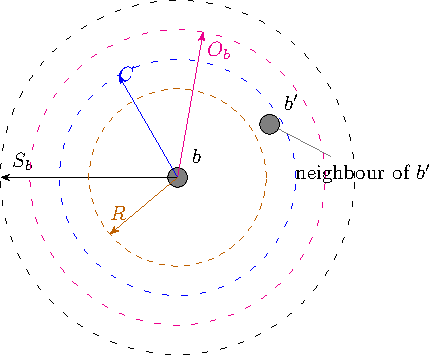
\includegraphics[width=0.5\linewidth]{figures/stableswarm}
	\caption[Agent Fields]{Agent Fields}
	\label{fig:stableswarm}
\end{figure}

\section{Resultant Vector Calculation}
In the Original work by Eliot et. al. the resultant vector of an agent was calculated using Equation~\ref{eq:resultantVector}. Where $k_c,k_r,k_d,k_o$ are weighting factors for the summed vectors associated with each interaction. The new algorithm requires each individual agent to have a variation to the vector generated inside each calculation based on the perimeter status of the agent and each neighbour. The equation therefore needs to have an additional weighting factor applied to specific agents within the cohesion and repulsion vector calculations ($k_{cpc}$,$k_{rpc}$) as shown is Equation~\ref{eq:newResultantVector}).

\begin{equation}\label{eq:resultantVector}
	v(b) = k_cv_c(b) + k_rv_r(b) + k_dv_d(b) + k_ov_o(b)
\end{equation}
	
\begin{equation}\label{eq:newResultantVector}
	v(b) = k_cv_c(b,k_{cpc}) + k_rv_r(b,k_{rpc}) + k_dv_d(b) + k_ov_o(b)
\end{equation}

the effects of the addition of these additional weighting factors can be seen in Figure~\ref{fig:compressioneffect1}. The metric used in producing the graph is based upon the inter-agent magnitudes~\cite{eliot2018metric}.

\begin{figure}[h]
	\centering
	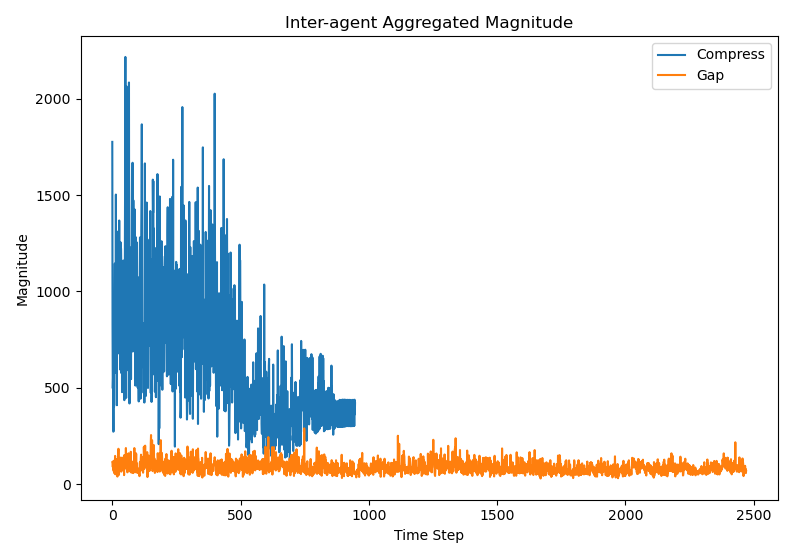
\includegraphics[width=0.75\linewidth]{figures/CompressionEffect1}
	\caption[Compression Effect]{Compression Effect based on Magnitude change}
	\label{fig:compressioneffect1}
\end{figure}


\section{Repulsion}\label{repulsion}
The repulsion component of an agent's movement is calculated from its interaction with its neighbours $nbr(b)$ that are within the agent's ($b$) repulsion field ($R_b$) (Eq.~\ref{eq:Repulsion1}) or from any agent in the swarm ($S$) that are within the agent's ($b$) repulsion field ($R_b$) (Eq.~\ref{eq:Repulsion2}). The resultant set will be the same.\\

\begin{equation}\label{eq:Repulsion1}
R(b) = \{b' \in S~:~\magn{bb'} <= R_b\}
\end{equation}

Given that the repulsion field is within the cohesion field (neighbours) then the repulsion set can also be identified as a subset of those neighbours where $nbr(b)$ is the set of all of the neighbours of $b$ \cite{eliot2017methods}:

\begin{equation}\label{eq:Repulsion2}
R(b) = \{b' \in nbr(b)~:~\magn{bb'} <= R_b\}
\end{equation}

\subsection{Compression repulsion}

\begin{assumption}
	$k_{rpc} <= 1$
\end{assumption}

To reduce the repulsion effect, the control factor ($k_{rpc}$) is applied to an agent's repulsion field if both itself and it's neighbour are perimeter agents. Where $per()$ returns an agent's perimeter status. An agent is identified as a perimeter agent using the technique shown by Eliot et.al. in \cite{eliot2019void}

Therefore if the condition of both agents being a perimeter is met ($per(b)\wedge per(b')$), where $per()$ returns $true$ if an agent is on the perimeter and or $false$ if it is not, and $b'$ is within repulsion field distance multiplied by the compression factor, or both agents are not both perimeter agents ($\neg(per(b)\wedge per(b'))$) and $b'$ is within the `normal' repulsion field ($R_b$) then an agent is part of the repulsion set (Eq. \ref{eq:Repulsion3} or \ref{eq:Repulsion4})

\begin{flalign}\label{eq:Repulsion3}
\begin{split}
R(b) = & \{b' \in S~:\\
&(per(b)\wedge per(b')\wedge\magn{bb'} <= k_{rpc}R_b) \\
&\vee\\ 
&(\neg(per(b)\wedge per(b'))\wedge\magn{bb'} <= R_b)\\
&\}
\end{split}
\end{flalign}

or

\begin{flalign}\label{eq:Repulsion4}
\begin{split}
R(b) = & \{b' \in nbr(b)~:\\
&(per(b)\wedge per(b')\wedge\magn{bb'} <= k_{rpc}R_b) \\
&\vee\\ 
&(\neg(per(b)\wedge per(b'))\wedge\magn{bb'} <= R_b)\\
&\}
\end{split}
\end{flalign}

The effect of either is that perimeter-based agents will be allowed to be closer together before a repulsion vector is generated. 

\important{The repulsion vector that is generated is based upon the $R_b$, the full repulsion field, and not the reduced field. This is to reduce potential agent collisions.}

\section{Cohesion}\label{cohesion}

\begin{assumption}
	$k_{cpc} >= 1$
\end{assumption}

To be completed.

\section{Conclusions}\label{conclusions}
From the initial simulations it is possible to show that the technique is able to successfully remove voids and surround an obstacle as shown in the video \href{https://youtu.be/3eY1vvq0JWo}{https://youtu.be/3eY1vvq0JWo}.

\bibliographystyle{abbrv}
\bibliography{perimeter}

\end{document}